\graphicspath{ {Figures/TMethod/ResidualsFFT/} }

\chapter{T Method Fit}
\label{Ch:TMethod}

This entire chapter is a work in progress.


While not the main focus of my analysis, I also perform a T-Method fit to the data along with the ratio fit. This is useful as a comparison to the ratio method results, and can also provide useful parameter information that the ratio method has trouble getting at. I do not perform systematic studies, and only perform further analysis checks like fit start time scans to verify that the T-Method fit is working correctly. In my T-Method fit, I include all CBO terms, the vertical waist, and lost muons, as described in Chapter \ref{Ch:Procedures}. The same fit start and end times as used in the ratio fit ($\SI{30}{\mu s} - \SI{650}{\mu s}$) are used here as well.

The results for a T-Method fit are shown in Figure 

A table of the results with parameter information is shown in Table \ref{Tab:FitParamsTMethod}

The correlation matrix for the T-Method fit is shown in Table

An FFT of the results is included for posterity in Figures 



A comparison between the ratio and T-Method results are shown in Table

There is a slight difference in data that is fitted between the T method and the ratio method. Because of the time shifting that is done in the ratio method, there is a quarter \gmtwo periods worth of data starting at $\SI{30}{\mu s}$ that is replaced by data before $\SI{30}{\mu s}$. This shouldn't change much but should be kept in mind when comparing...



	\begin{table}[]
	\centering
	\setlength\tabcolsep{10pt}
	\renewcommand{\arraystretch}{1.2}
	\begin{tabular*}{.8\linewidth}{@{\extracolsep{\fill}}|l|l|c|c|}
	  \hline
	  	\multicolumn{4}{|c|}{\textbf{T-Method Fit Results}} \\
	  \hline\hline
	  	\multicolumn{2}{|c}{$\chi^{2}$/NDF}       				&  \multicolumn{2}{c|}{$2964/3137$}  \\
	  	\multicolumn{2}{|c}{P value}         	 				&  \multicolumn{2}{c|}{$0.9867$}  \\
	  \hline\hline
	  	Parameter & Descriptor & Value & Error \\
	  \hline
		$N_{0}$    			  & Number  	    			&  $\SI{3.327e6}{}$  	&	$\SI{2.668e2}{}$  \\
		$\tau$    			  & Muon Lifetime $(\mu s)$ 	&  $64.44$  			&	$\SI{3.965e-3}{}$  \\
		$A$    			 	  & Asymmetry  	    			&  $0.3704$  			&	$\SI{4.493e-5}{}$  \\
		$R$     			  & R (ppm, blinded)   	 		&  $-19.88$  			&	$1.373$  \\
		$\phi$   			  & \gmtwo Phase         		&  $2.091$  			&	$\SI{2.249e-4}{}$  \\
		$\omega_{cbo}$   	  & CBO Frequency $(MHz)$       &  $0.37$  				&	$\SI{}{}$  \\
		$\tau_{cbo}$          & CBO Lifetime $(\mu s)$ 	    &  $182.1$  			&	$15.67$  \\
		$A_{cbo-N}$   	 	  & CBO N Amplitude      		&  $0.00449$  			&	$\SI{2.365e-4}{}$  \\
		$\phi_{cbo-N}$   	  & CBO N Phase       	 		&  $-1.835$  			&	$0.1017$  \\
		$A_{cbo-A}$   	 	  & CBO A Amplitude      		&  $0.00449$  			&	$\SI{2.365e-4}{}$  \\
		$\phi_{cbo-A}$   	  & CBO A Phase       	 		&  $-1.835$  			&	$0.1017$  \\
		$A_{cbo-\phi}$   	  & CBO $\phi$ Amplitude      	&  $0.00449$  			&	$\SI{2.365e-4}{}$  \\
		$\phi_{cbo-\phi}$     & CBO $\phi$ Phase       	 	&  $-1.835$  			&	$0.1017$  \\
		$\omega_{VW}$   	  & VW Frequency $(MHz)$        &  $2.3$  				&	$\SI{}{}$  \\
		$\tau_{VW}$           & VW Lifetime $(\mu s)$ 	    &  $18$  				&	$15.67$  \\
		$A_{cbo-VW}$   	 	  & VW Amplitude      			&  $0.001$  			&	$\SI{2.365e-4}{}$  \\
		$\phi_{cbo-VW}$   	  & VW Phase       	 			&  $-0.34$  			&	$0.1017$  \\
		$\kappa_{loss}$   	  & Lost Muon Normalization     &  $6.7$  			    &	$2$  \\
	  \hline
	\end{tabular*}
	\caption{Table of T-Method fit results.}
	\label{Tab:FitParamsTMethod}
	\end{table}





	\begin{figure}[h]
	\centering
	    \begin{subfigure}[]{0.45\textwidth}
		    \centering
			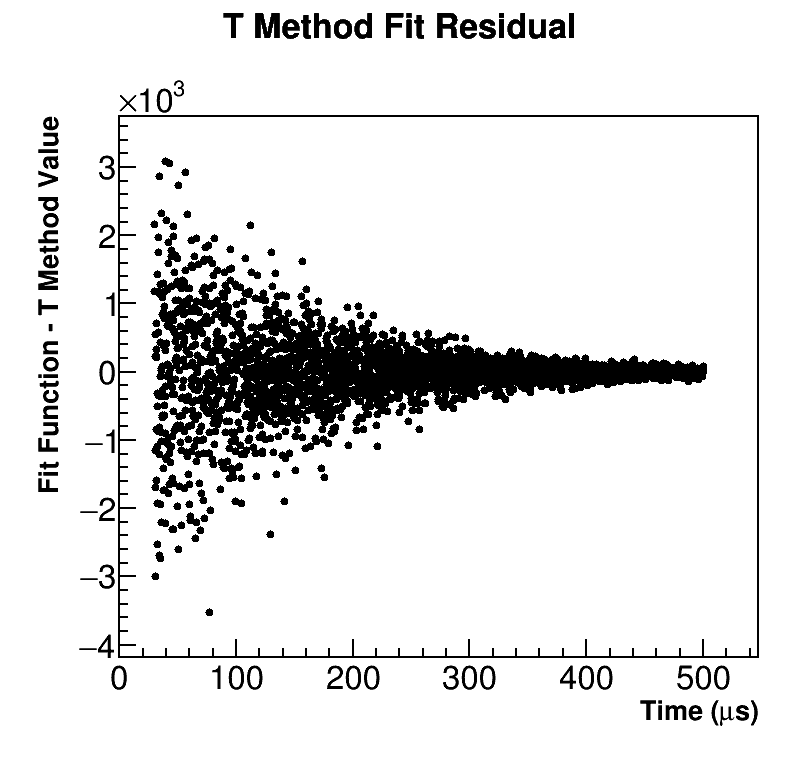
\includegraphics[width=\textwidth]{fitResidual_TMethod}
		    \caption{Fit residuals.}
	    \end{subfigure}
	    \begin{subfigure}[]{0.45\textwidth}
		    \centering
			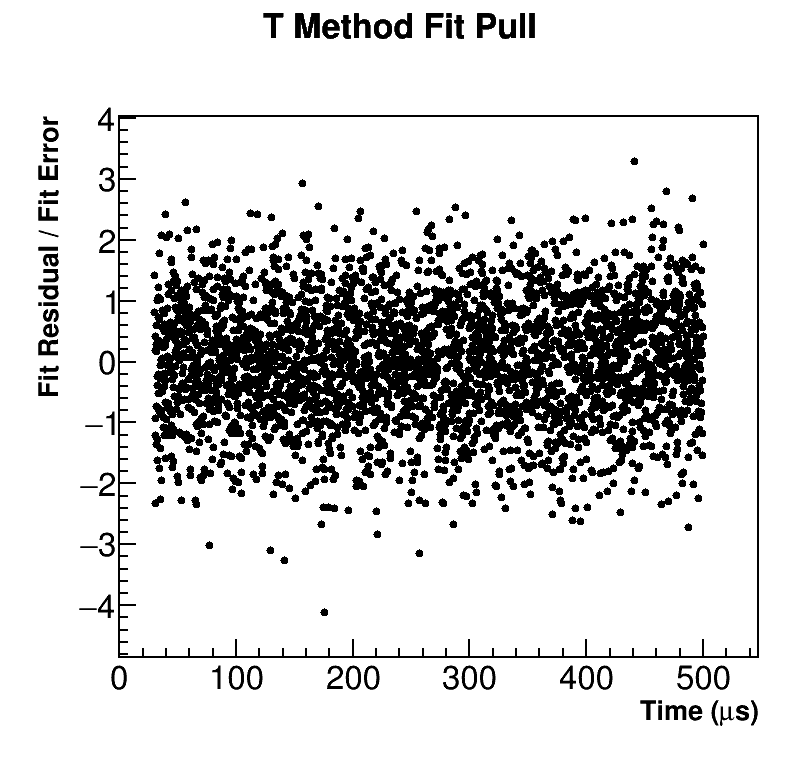
\includegraphics[width=\textwidth]{fitPull_TMethod}
		    \caption{Fit pulls.}
	    \end{subfigure}% %you need this % here to add spacing between subfigures
	    \vspace{4mm}
	    \begin{subfigure}[]{0.7\textwidth}
		    \centering
			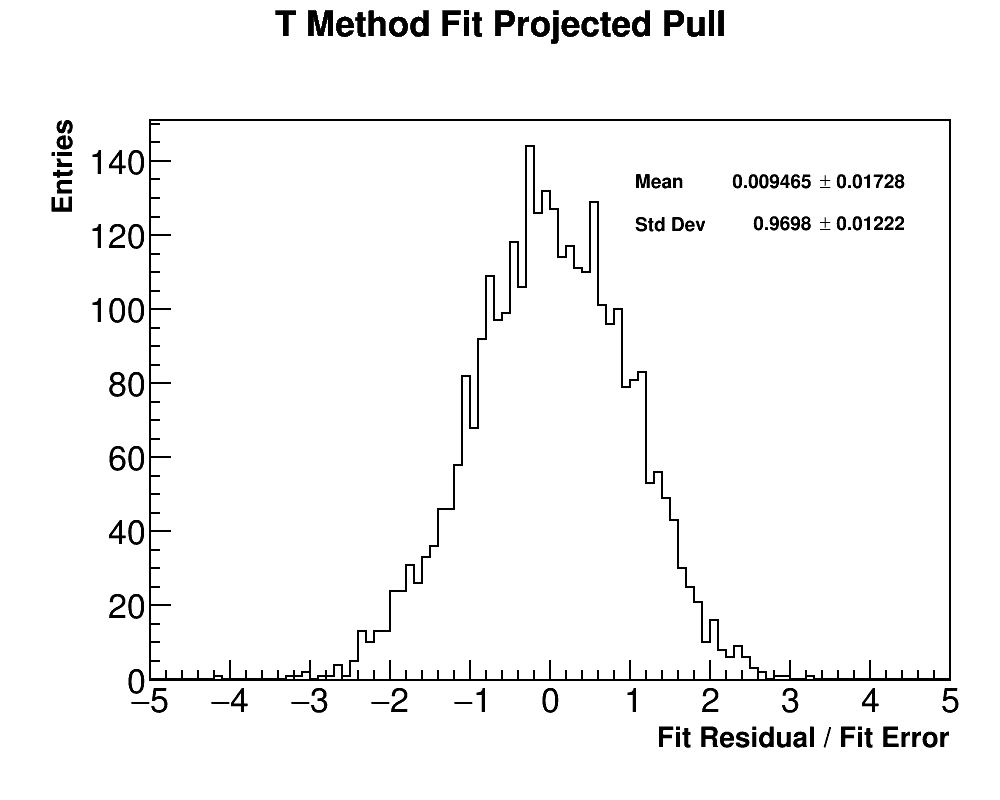
\includegraphics[width=\textwidth]{fitPull_projected_TMethod}
		    \caption{Fit pulls projected onto the y axis. Note the Gaussian shape centered around 0 with unit width.}
	    \end{subfigure}
	\caption[fitResidual_TMethod]{Residuals and pulls for the T Method fit.}
	\label{fig:fitResidual_TMethod}
	\end{figure}

	\begin{figure}[]
		\centering
		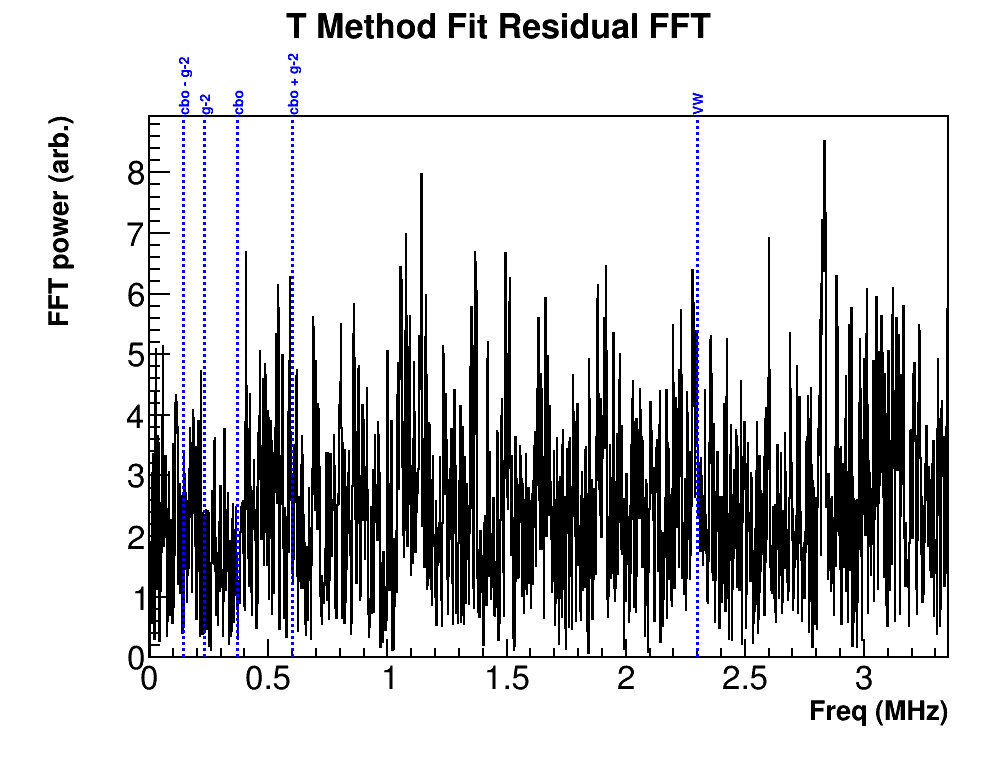
\includegraphics[width=\textwidth]{FFT_TMethodFit}
	    \caption[FFT_TMethodFit]{FFT of the residuals of the T Method fit. No significant peaks remain in the fit residuals after fitting with all terms. Overlayed are dotted lines for the \gmtwo, CBO, and vertical waist frequencies.}
	    \label{fig:FFT_TMethodFit}
	\end{figure}

	\begin{figure}[]
		\centering
		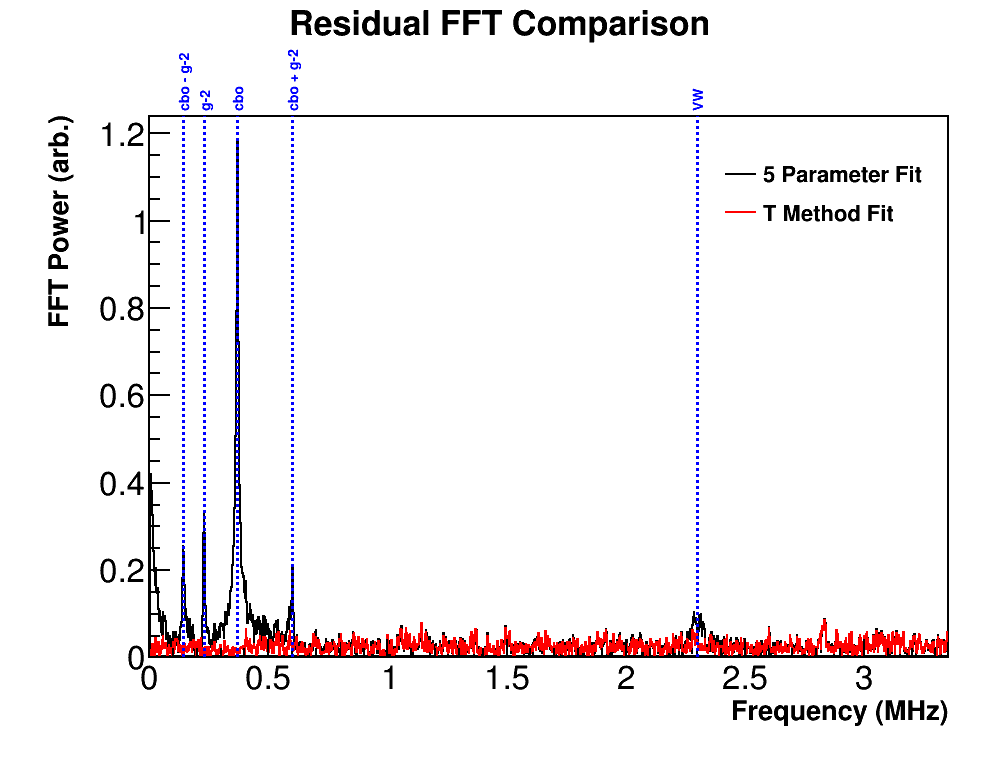
\includegraphics[width=\textwidth]{FFTComparison_TMethod}
	    \caption[FFTComparison_TMethod]{A plot of the FFT of the residuals of the fit for the five parameter fit compared to the T Method fit. In black is the FFT for a five parameter fit, where peaks for the CBO and vertical waist can be seen as well as the \gmtwo peak. In red is the FFT of the T Method fit residuals.}
	    \label{fig:FFTComparison_TMethod}
	\end{figure}






\section{Toy MC Comparison}


In order to assist in combining the ratio method results with those of the other analyzers and their T method results, it's useful to perform MC comparison between the ratio and T method fits. To do this I generated a set of ``positron'' toy MC data using a 1D \texttt{ROOT} function, corresponding to an energy threshold time histogram. The times of these hits were randomized in the same way as done for data to remove the fast rotation. These times were also randomly split into the separate U and V histograms to form the ratio. 5 parameter and 3 parameter ratio fits were then performed on the created histograms, and the subsequent fitted R values were put into separate histograms. The randomizations for the times and UV filling were then done 50 times to generate two histograms of fitted R values for the 5 parameter and 3 parameter ratio fits respectively. 
In this way a single pseudo-experiment for a single set of ``positron'' data for a number of seeds was performed. The results for these two histograms is shown in Figure blank. The difference between the two means of these R histograms were then put into another histogram, a histogram of the mean difference between the fitted R values between the two types of fits for a single pseudo experiment. Finally, the whole process was repeated 100 times for 100 pseudo experiments, to fill out the mean difference histogram. It is this histogram that gives a measure of the expected difference between the fitted R results for the T method fit and the ratio method fit in data. This is shown in Figure blank.




Do I want to include my T method data randomization results as well here or somewhere in this chapter?












